\subsection{Thermal History and Present Thermal State}
The thermal evolution of Mars and its present thermal state cannot be assessed by direct measurement. Rather, the thermal history needs to be reconstructed from the thickness of the crust, the timing and distribution of surface volcanism as well as the erupted volume over time, petrological and isotope data of the Martian meteorites, and estimates of the elastic lithosphere thickness. In addition, the evolution of the atmosphere and the magnetic properties of the planet need to be considered. The InSight mission will complement these data by providing a measurement of the surface heat flow at the landing site that has a good chance of being representative of the average surface heat flow \citep{Plesa2016} of the planet. Numerical model calculations of the thermal evolution and the present thermal state offer valuable insights into the interior of the planet and can be used to integrate the observational data into a coherent model. In this section, we discuss the thermal evolution of Mars and present reference models of its present thermal state.

A number of numerical studies using either parametrized models or 2D and 3D fully dynamical simulations of mantle convection have been employed to investigate the thermal evolution of Mars \citep[for a recent review see][]{BreuerMoore2015}. While the parameterized models rely on appropriate scaling laws of convective heat transport to compute average values of quantities such as temperature and crustal thickness, 2D and 3D calculations numerically solve the full set of conservation equations of mass, momentum and thermal energy. The advantage of parametrized models is that they can span a large set of parameters and initial conditions for which fully dynamical simulations may require excessive amounts of computational time. However, albeit computationally fast, parametrized models cannot self-consistently resolve spatial variations caused by e.g., mantle plumes and crust thickness variations and for this, 2D and 3D fully dynamical models are better suited.
\subsubsection{Crust formation, crust and mantle chemical reservoirs}
\label{Crust formation}
The timing of volcanic activity and amount of crustal production as well as volcanic outgassing and magnetic field history have been mostly investigated with parametrized thermal evolution models \citep[e.g.,][]{Hauck2002, Breuer2003, Breuer2006, Schumacher2006, Fraeman2010, Morschhauser2011, Grott2011} although this topic has been addressed also in 2D and 3D studies \citep[e.g.,][]{Ruedas2013, Plesa2014a, Sekhar2014}. The models predict an intense episode of mantle melting and crust formation early in the planetary evolution (i.e., during the Noachian and early Hesperian) and are consistent with the observations if a wet mantle rheology and a comparatively low initial temperature are used \citep[e.g.,][]{Hauck2002, Breuer2006, Fraeman2010, Morschhauser2011, Grott2011}. Although a dry mantle rheology with a primordial crust and higher initial mantle temperature would also be consistent with the inferred crustal history \citep{Breuer2006}, such models cannot be reconciled with the small elastic lithosphere thickness values inferred for the Noachian epoch from lithosphere deformation studies \citep{Grott2008, Grott2013}. A recent study, using 3D thermal evolution models showed that a dry mantle rheology can explain the small elastic thickness during the Noachian but in this case a wet crustal rheology must be assumed \citep{Breuer2016}. The large present-day elastic lithosphere thickness at the north pole of Mars necessarily requires a dry mantle rheology today, however. This suggests that the Martian mantle may have contained a rheologically significant amount of water, which has been partly or entirely lost by outgassing over time while  the Martian crust must have been rheologically wet at least during the Noachian period.   

The volcanic activity of Mars rapidly declined during the Hesperian and Amazonian and became restricted to the large volcanic provinces in Tharsis and Elysium \citep[e.g., ][]{Greeley1981}. Numerical studies in 3D geometry show that accounting for mantle phase transitions, a pressure-dependent viscosity or a viscosity layering in the mid mantle, possibly associated with a mineralogical phase transition in the interior of Mars, can lead to a low degree convection pattern, which may produce the observed crustal dichotomy and explain long-standing volcanic activity in Tharsis and Elysium \citep[e.g.,][]{Harder1996, Breuer1998, Zhong2001, Roberts2006, Keller2009, Sramek2010}. 
A dynamic link between the early evolution of Tharsis and the crustal dichotomy has been also suggested as a result of the formation of a thick lithospheric keel underneath the southern hemisphere \citep{Zhong2009,Sramek2012}. This lithospheric keel may represent the melt residue after the dichotomy formation process and, if sufficiently thick, cause the rotation of the entire lithosphere with respect to the underlying mantle, which explains the migration of the Tharsis volcanic center to the dichotomy boundary. However, dynamical models considering the formation of the crustal thickness dichotomy and Tharsis investigate only the first billion year of thermal history, and whether such models will continue to experience significant volcanic activity thereafter is still not clear. A significant amount of melt produced during later stages of evolution would be inconsistent with estimates of the crustal production rate on Mars \citep{Greeley1991}.

Models of mantle convection in 2D and 3D geometry are also a natural choice for studies of the interior dynamics of Mars, which investigate the formation and stability of geochemical reservoirs, as suggested by the isotopical analysis of Martian meteorites \citep[e.g.,][]{Jagoutz1991}. Although previous studies argued for the formation of mantle reservoirs during the crystallization and subsequent overturn of a global magma ocean \citep[e.g.,][]{Elkins-Tanton2003, Elkins-Tanton2005}, recent studies suggest that such heterogeneities could have been largely or even entirely erased if solid-state mantle convection started before the complete crystallization of the magma ocean \citep{Maurice2017}. Alternative scenarios suggest that the formation of mantle geochemical anomalies could be explained by partial melting of an initially homogeneous mantle, if additional effects like density variations and mantle dehydration are considered \citep[e.g.,][]{Schott2001, Ogawa2011, Plesa2014a, Ruedas2017}. As the planet cools, the stagnant lid (i.e., the immobile layer that forms at the top of the convecting mantle due to the strong temperature dependence of the viscosity) grows. Geochemical reservoirs if located close to the surface, may become trapped within the stagnant lid and remain protected from mixing and homogenization that otherwise would take place in a vigorously convecting mantle \citep[e.g.,][]{Breuer2016}. If on the other hand, the liquid magma ocean rapidly crystallized and no mixing took place prior to complete solidification, numerical modeling studies suggest that the density contrasts established during magma ocean crystallization would be too strong to allow the later onset of thermally driven convection \citep{Tosi2013, Plesa2014}. Such a scenario is at odds with the volcanic history on Mars and also with the thin elastic lithosphere of about 20 km inferred for the Noachian epoch (see below), which requires a thin thermal boundary layer and consequently a vigorously convecting mantle at that time.

\subsubsection{Radiogenic Element distribution in crust, mantle and core}
The long-lived radiogenic isotopes (K, Th, and U) are the primary sources of heat in the interior of Mars. Estimates of their concentrations in the primitive mantle come from geochemical models \citep[][see also section 2.2]{Dreibus1984, Wanke1994, Treiman1986, Morgan1979, Lodders1997}. Most compositional models predict similar amounts of Th but substantially different potassium abundances. Only the model by \citet{Morgan1979} has almost twice as much Th and a significantly smaller amount of K. In addition, they used a low ratio of K/U of 2200 as determined from gamma spectrometric analysis performed by the Soviet orbiter Mars 5. This value was later corrected by the gamma-ray spectrometer (GRS) data obtained by Mars Odyssey. The surface ratio of K/Th measured by the GRS instrument varies for 95\% of the surface area between 4000 and 7000 \citep{Taylor2007} and is largely consistent with the preferred compositional model of \citet{Wanke1994}.  Today the heat sources are not homogeneously distributed in the Martian interior because these incompatible elements are preferentially sequestered into a planet's crust during differentiation \citep{Taylor2008}. Alternatively, \citet{Kiefer2003} argues that recent volcanism could be driven by radiogenic material in the mantle. To estimate the abundance in the crust, in-situ measurements by landers and rovers, remote measurements from orbiting spacecraft, and meteorite samples have been used \citep[e.g.,][]{Taylor2007}
\begin{table}[h!]
\centering
\label{table2}
\resizebox{\textwidth}{!}{
\begin{tabular}{llllll}
                              & U (ppb) & Th (ppb) & K (ppm)  & H\textsubscript{0} (pW/kg) & H\textsubscript{today} (pW/kg) \\
Model                         &         &          &          &            &                \\
Treiman et al. (1986)         & 16      & 64       & 160      & 17         & 3.7            \\
Morgan and Anders (1979)      & 28      & 101      & 62       & 21         & 5.6            \\
Wänke and Dreibus (1994)           & 16      & 56       & 305      & 23         & 4.1            \\
Lodders and Fegley (1997)     & 16      & 55       & 920      & 49         & 6.2            \\
Basaltic Shergottites*+       & 26--184  & 100--700  & 200--2600 & --      & 5.9 -- 45.5     \\
GRS data                      & 163     & 620      & 3300     & --         & 49             \\
(average surface abundances)* &         &          &          &            &               
\end{tabular}
}
\caption{Abundance of heat-producing elements in the primitive mantle for various compositional models, SNC meteorites and average surface crustal composition measured by GRS and corresponding heat production at the beginning of the evolution (H\textsubscript{0}) and after 4.5 Ga (H\textsubscript{today}). *The U abundances are determined by assuming a Th/U ratio of 3.8, a canonical cosmochemical value thought to be representative of most planetary bodies and that also agrees with analyses of most Martian meteorites \citep{Meyer2003}.+ Most of the basaltic shergottites show values close to the lower bound.}
\end{table}

The GRS data do not present evidence for significant large-scale geochemical anomalies \citep{Hahn2011} and the surface distribution of Th only shows slight variations between 0.2 and 1 ppm \citep{Taylor2007}. Assuming the compositional model of Dreibus and W\"anke and further assuming that the composition of near surface rock reflects the average crustal composition, thus neglecting any intracrustal differentiation, the percentage of heat producing elements (HPE) in the crust is between 29\% and 70\% of the total \citep{Taylor2007}.  The uncertainty in this estimate is being caused by the unknown crust thickness (see section 2.3). This estimate further implies that most of the Martian crust was derived from an undepleted mantle and that the concentrations of K and Th in the bulk crust are higher than in the basaltic Martian meteorites (see Table 2) and in the basaltic rocks analyzed by the MER rovers \citep[e.g.,][]{ McLennan2001}. The latter rock samples would then need to have been derived from a depleted mantle. An alternative scenario is that a significant portion of the crust does consist of basaltic rocks relatively low in K and Th, similar to the Martian meteorites, and that the observed soil composition represents a reservoir enriched in incompatible elements relative to the bulk of the basaltic crust. In that case, the surface composition from the GRS data represents an upper limit to the abundance of HPE in the crust \citep{Newsom2007}. Assuming the W\"anke-Dreibus abundance, this would imply that only about 10\% of Th and K are partitioned into the crust, or that bulk Mars has lower abundances of Th and K.  Thermo-chemical evolution models favor the former model as this will better explain the inferred large elastic lithosphere thickness at the north pole and the recent volcanic activity (\cite{Kiefer2003}, also see section 3.1.3). 

The distribution of HPE in the mantle is basically unknown. Often, it is assumed that HPE are homogeneously mixed due to mantle convection. However, mantle melting and differentiation may lead to reservoirs of varying abundances and in particular the lower part of the stagnant lid and/or an upper mantle layer can be depleted in HPE in comparison to the lower mantle \citep{Ruedas2013, Plesa2014a}. 
The compositional models generally assume no radiogenic heat sources in the core. However, this is controversially discussed because recent experimental results suggest that K may partition into the core at the relatively low pressures and high sulfur contents appropriate to Mars \citep{Murthy2003}.

\subsubsection{Surface heat flow and the Urey ratio}
\label{Te_heat_flow_Urey}



Models of thermal evolution in a 3D geometry employing a crustal thickness whose spatial variations are consistent with gravity and topography data \citep[e.g.,][]{Neumann2004} and a crustal enrichment that matches the surface abundance of heat producing elements \citep{Taylor2007, Hahn2011} indicate elastic thickness values close to 300 km at the north pole and as small as 42 km in Arsia Mons (Figure 7a). Such low values suggest that a decoupling layer in the lower crust is still present today in this region \citep{Grott2010, Plesa2016}. The low elastic thicknesses during the Noachian period can be explained if a weak crustal rheology is assumed \citep{Grott2008, Breuer2016}. The evolution of the elastic lithosphere thickness predicted by the 3D thermal evolution models, accounting for a weak crustal rheology and mantle plumes, is shown in Figure 7b. These models show a spatial distribution of the surface heat flow, which is dominated by the crustal thickness pattern \citep{Plesa2016} and attains the smallest values in regions covered by a thin crust (e.g., Utopia, Hellas, Agyre and Isidis impact basins), while the largest values are obtained for regions covered by a thick crust (e.g., Tharsis province). A crustal thickness dichotomy leads to higher surface heat flow values for the southern highlands compared to the northern lowlands. If instead the crustal thickness variations are reduced by assuming a variable crustal density, the surface heat flow shows a rather homogeneous distribution \citep{Plesa2016}. The signature of mantle plumes may become visible on the surface heat flow maps if an activation volume of 10 cm$^3$/mol is considered, which leads to a strong increase of viscosity with pressure of about two orders of magnitude. Nevertheless, for a variety of parameters, the models predict that the location of mantle plumes is unlikely to affect the heat flow measurement. The difference between the heat flow value that will be obtained by the HP$^3$ instrument and the average surface heat flow will be less than 5 mW/m$^2$ \citep{Plesa2016}. This suggests that InSight will return a representative value for the average surface heat flow.

\begin{figure}[h!]
\begin{center}
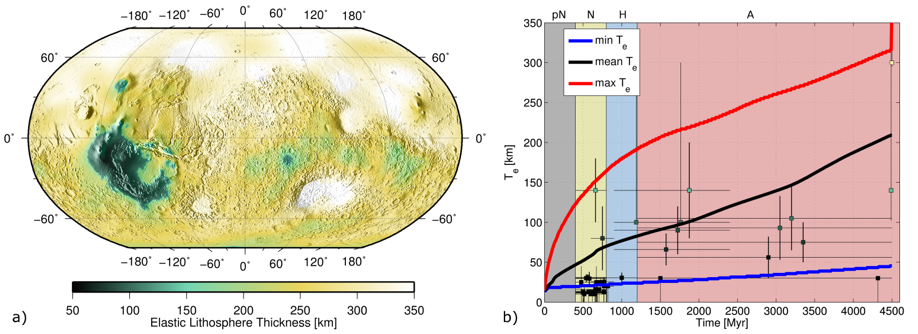
\includegraphics[width=\textwidth]
{figures/Fig3.png}
\caption{Elastic lithosphere thickness: a) Spatial distribution of the present-day elastic lithosphere thickness calculated using a strain rate of $10^{-14}$ s$^{-1}$ which is characteristic for the timescale associated with the polar cap deposition at the north pole of Mars; b) Evolution of the elastic lithosphere thickness that was computed assuming a strain rate of $10^{-17}$ s$^{-1}$, which is representative for convection timescales, for the entire evolution apart from the maximum value today. The latter has been calculated using the strain rate value of $10^{-14}$ s$^{-1}$. The colored boxes represent the elastic lithosphere thickness estimates with their corresponding error bars.}
\label{fig:Fig3.png} 
\end{center}
\end{figure}

The average surface heat flow is an important quantity which can be directly related to the bulk abundance of HPE in the silicate part of the planet (mantle and crust) by using the so-called Urey ratio, which is defined as the ratio between the heat produced by radioactive elements in the silicate part and the heat loss over the surface. Numerical simulations show that as long as the mantle of Mars is efficiently convecting, the Urey ratio converges towards a similar present-day value independent of mantle parameters such as e.g., initial mantle temperature and the distribution of heat sources between crust and mantle \citep{Grott2012a, Plesa2015}. Thus by using the average surface heat flow, which will be derived from the InSight measurement, together with the Urey ratio, that is calculated from thermal evolution models, one can estimate the bulk abundance of HPE in the interior of Mars and answer the fundamental question as to whether the amount of heat producing elements in the interior of the planet is \revision{similar to previously proposed geochemical models \citep{Wanke1994,Lodders1997,Treiman1986} or lower \citep{Phillips2008}.}

\subsubsection{Reference Temperature Profile -- A Geotherm }
\label{ref_temp}
In this section we will present a reference thermal model for the interior of Mars based on the mantle convection calculations discussed above. The 3D calculations have been introduced elsewhere in greater detail \citep[e.g.,][]{Plesa2016} and will therefore only be briefly described here. The calculations are based on the extended Boussinesq assumption \citep[e.g.,][]{Schubert2001} for which the temperature and pressure dependencies of material parameters are accounted for in the buoyancy term and for which adiabatic and viscous heating are included. In addition, the models use a pressure- and temperature-dependent rheology, with a reference viscosity evaluated at 3 GPa and 1600 K. The calculations assume a crust that has been differentiated from the mantle. We use the \citet{Neumann2004} crustal thickness model as well as other models as discussed in section 2.3 derived from MGS gravity measurements. The crust is enriched in radiogenic elements as compared to the mantle. The enrichment factor is 10 with respect to the bulk value and is consistent with the surface concentrations measured by the gamma ray instrument on board Mars Odyssey \citep{Taylor2007, Hahn2011}. The concentration of the radiogenic elements is considered constant for simplicity although it has long been argued that it may vary with depth \citep[e.g.,][]{Newsom2007}. In addition to the 3D temperature in the mantle and crust, the model provides maps of the elastic thickness of the lithosphere and the surface heat flow. Table 3 summarizes parameter choices made for the model. Note that we do not include a detailed model of the core. The likely low viscosity of the core precludes the use of a code tailored for mantle convection to model core flow. Rather, we solve an energy balance for the core in which the time rate of change of the core internal energy is balanced by the heat flow into the mantle integrated over the core surface and we extend the temperature from the core-mantle-boundary (CMB) into the core assuming a heat conduction profile discussed below. 
%

\begin{table}[h!]
\caption{Parameters used for the end-member models and the reference model. All models assume a core size of 1700 km and hence include only the exothermic phase transitions from $\alpha$ to $\beta$-spinel and $\beta$ to $\gamma$-spinel but no endothermic phase transition from $\gamma$-spinel to perovskite. \revision{All models use an activation energy of 300 kJ/mol. }For additional parameters we refer the reader to \citep{Plesa2016, Plesa2015} and \citep{Breuer1998}.}
\label{table:end_member_ref_models}

\begin{tabular}{ p{11em} p{2.5cm} p{2.5cm} p{2.5cm} }
\hline
\multirow{3}{12em} & Hot end-member model & Cold end-member model & Reference model \\
\hline 
Planetary radius {[}km{]} & 3400     & 3400    & 3400\\
Core radius {[}km{]} & 1700 & 1700 & 1700  \\
Reference viscosity {[}Pa s{]} & 1021 & 1020 & 1021 \\
Activation\_volume {[}cm$^3$/mol{]} & 0 & 10 & 10 \\
Crustal thickness model & {[}Neumann et al., 2004{]} & 3200\_1\_DWTh2Ref1 & 3100\_1\_DWTh2Ref1 \\
Depth of $\alpha$ to $\beta$-spinel 
phase transition {[}km{]}  & 1020 & 1020 & 1020 \\
Depth of $\beta$ to $\gamma$-spinel
phase transition {[}km{]} & 1360 & 1360 & 1360   
\end{tabular}
\end{table}

\revision{
The thermal models discussed below do not self-consistently account for Tharsis formation. The latter could have been formed by a low degree convection pattern \citep[e.g.,][]{Zhong2001,Roberts2006,Zhong2009,Sramek2010} or a large-scale impact onto the southern hemisphere followed by a degree-1 convection pattern \citep[e.g.,][]{Golabek2011,Golabek2018}. Whether the amount and distribution of crust produced in such scenarios would be compatible with the range of crustal thicknesses derived from gravity and topography data is still not clear. Since most of the martian crust has formed during the first 500-700 Myr of evolution \citep[e.g.,][]{Greeley1991}, the crustal thickness pattern and the crustal enrichment in heat producing elements could have influenced the underlying temperature distribution over several Gyr. By combining crustal thickness variations derived from gravity and topography data with thermal evolution models of interior dynamics and taking into account a number of observational data sets, we discuss a range of temperature variations that could be representative for the present-day interior of Mars.}

The crustal thickness pattern and the crust radioactivity cause spatial temperature variations in the shallowest layers, while deeper in the mantle thermal anomalies reflect the mantle flow pattern, which -- in turn -- is sensitive to the pressure and temperature dependence of the viscosity. \revision{The temperature and pressure dependence of the viscosity are determined by the activation energy and activation volume, respectively, and uncertainties of the activation parameters lead to uncertainties of temperature variations in the mantle. In particular, the large range of values obtained from deformation experiments of upper mantle rocks for the activation volume, i.e., 0--10 cm$^3$/mol for diffusion creep and even larger for dislocation creep \citep{Hirth2003}, indicate an increase of viscosity with pressure ranging from 0 to several orders of magnitude for Earth's upper mantle \citep{King2016} and would lead to significantly different convection planforms}. A strong increase of viscosity with pressure induces a long wavelength convection pattern with prominent mantle plumes that can considerably affect the temperature distribution and locally vary the thickness of the thermal boundary layer \citep[e.g.,][]{Yoshida2006, Roberts2006, Bunge1996}. 

On the other hand, a comparatively mild increase of viscosity with pressure, leads to weaker thermal anomalies in the mantle and smaller perturbations of the thickness of the thermal boundary layer and hence smaller overall temperature variations (compare Figs. 8 and 10 below). Temperature variations are strongest at the base of the upper thermal boundary layer, where cold thermal instabilities originate and hot mantle plumes, rising from the core-mantle boundary, locally penetrate and erode the stagnant lid. Even for the weakest thermal anomalies, temperature variations in the lithosphere are around 200 K. Recent deformation experiments conducted at pressure and temperature conditions relevant to the mantle of Mars seem to favor an increase of the viscosity with pressure through the mantle of more than two orders of magnitude \citep{Raterron2017}, thus suggesting strong mantle plumes and variations of the lithosphere temperature by several hundred Kelvin.

In Figure 8, we present two end-member models showing the smallest and largest temperature variations as well as a reference model, to be discussed further below. Figure 8 gives slices of the temperature field for the reference and end-member models using a Robinson projection at depths of 50 km (in the upper lithosphere) to 1400 km (roughly 300 km above the CMB). The models have been selected from a large number of study cases discussed in \citet{Plesa2016}. The model with the smallest temperature variations (case 8 of \citet{Plesa2016}) has no pressure dependence of the viscosity and uses the crust thickness model of \citet{Neumann2004} (Fig. 8a). The crust density is 2900 kg/m$^3$ and the minimum thickness is 5 km in the Isidis basin while the average crust thickness is 45 km. In contrast, the largest temperature variations (Figure 8b) are obtained for a model (case 27 of \citet{Plesa2016} with a strong pressure dependence of the viscosity and using the crustal thickness model 3200\_1\_DWTh2Ref1 of \citet{Plesa2016}. The crust density is 3200 kg/m$^3$, the minimum crustal thickness is 1 km in Isidis, and the  average crustal thickness is 87 km for this model. 
%
\begin{figure}[h!]
\begin{center}
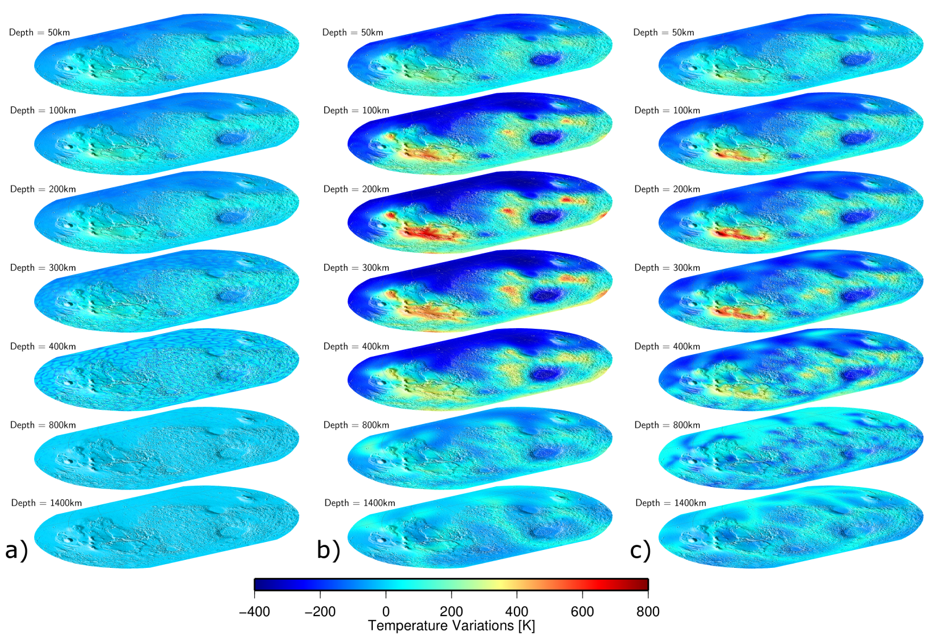
\includegraphics[width=\textwidth]
{figures/Fig4.png}
\caption{Present-day temperature variations in the Martian mantle: a) An end-member case showing the smallest variations (case 8 of \citet{Plesa2016}); b) An end-member case showing the largest variations (case 27 of \citet{Plesa2016}); c) The reference case (see text for details).}
\label{fig:Fig4.png} 
\end{center}
\end{figure}
%
The reference model has been selected by comparing our model results to a number of constraints from the Martian geologic record. As constraints we use the following observations: 
\begin{itemize}
\item	The present-day elastic thicknesses of the north and south polar lithosphere of more than 300 km and 110 km, respectively, as discussed above. In addition, the model is required to satisfy a Noachian elastic lithosphere thickness of 20 km \citep[][and references therein]{Grott2013} 
\item	Evidence for recent magmatic activity. Thus temperatures in the upper mantle must at least locally allow for partial melting. For the solidus of the mantle we use a recent compilation based on mineralogical models of the Martian mantle and available laboratory solidus temperatures \citep{Ruedas2017}.
\item	Petrological investigation of shergottites require potential temperatures in the mantle between 1480 and 1550°C around 180 -- 472 Myr ago \citep{Filiberto2015}. This observation constrains the mantle temperature to allow for at least local values in excess of the solidus temperature at the indicated times. 
\item	The potential of a model to relate the prominent topography features such as Tharsis and Hellas to mantle up- and downwellings

\end{itemize}

The model that best fits the constraints above, employs a large pressure dependence of the viscosity and a relatively thick crust. Other model parameters are taken from case 25 of \citet{Plesa2016}. The crust thickness model is 3100\_1\_DWTh2Ref1, with a crustal density of 3100 kg/m$^3$, a minimum crustal thickness of 1 km in the Isidis basin, and an average crustal thickness of about 62 km (Section 2.3). 

It can be seen that the maximum positive thermal anomalies are associated with Tharsis in both the reference and the end-member model with the largest temperature variations \revision{(Fig. 8)}. The particular thick and warm crust there that will attract mantle plumes causes this. Similarly, thin and cold regions of the crust, in particular Hellas, attract cold downwellings of mantle flow. Mantle plumes underneath Tharsis and Elysium are, of course, reasonable given the volcanic activity there that has lasted until recently \citep[e.g.,][]{Werner2009}. The figure also illustrates how the amplitudes of the thermal anomalies decrease with depth \revision{(Fig. 8)} to almost vanish near the CMB \revision{(Fig. 10)}.

\revision{In Figure 9 we show the present-day convection pattern obtained below Tharsis and Elysium in the reference model. }The model suggests that mantle plumes are present in the interior of Mars and are causing large spatial variations of the elastic thickness, surface heat flow and lithospheric temperatures (Figure 7 and 8). Large temperature variations may affect the seismic velocities in the shallowest layers of the planet up to 400 -- 500 km depth and hence may be detected by the SEIS instrument.
%
\begin{figure}[h!]
\begin{center}
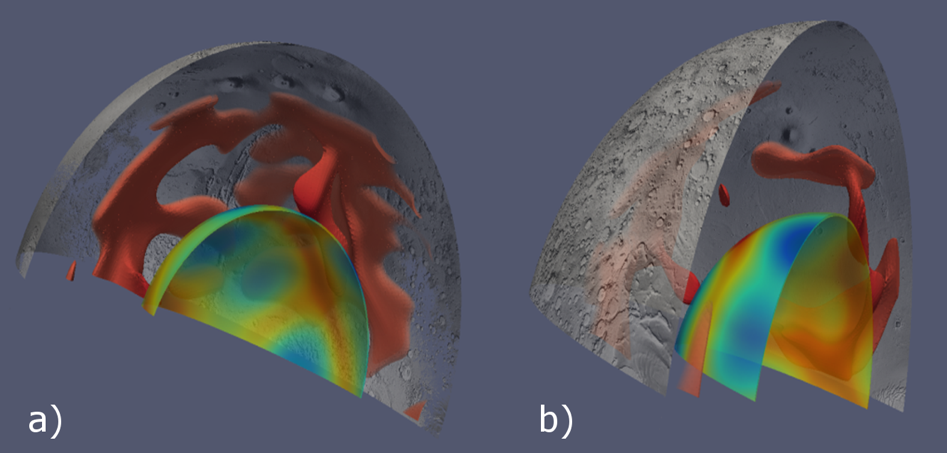
\includegraphics[width=\textwidth]
{figures/Fig5.png}
\caption{Present-day convection pattern in the interior of Mars: mantle plumes distribution below Tharsis (a) and Elysium (b) in the reference 3D thermal model.}
\label{fig:Fig5.png} 
\end{center}
\end{figure}
%

Figure 10a shows the reference temperature profile calculated from averaging over longitude and latitude at constant radial distance from the center in addition to profiles for the maximum and a minimum temperature anomaly cases introduced above. The models give the same surface heat flow value of about 24 mW/m$^2$ and a thermal lithosphere thickness of 450 to 600 km, respectively. In the thermal lithosphere, heat transfer is mostly by heat conduction and the temperature profile is comparatively steep. In the deeper mantle, the temperature profile bends over and is close to an adiabat at larger depth. For comparison, we present a mantle adiabat following \citet{Khan2018} that includes temperature jumps at mineralogical phase change boundaries. 

The deviations from the adiabat\revision{, which are observed in Figure 10a for temperature profiles obtained by 3D thermal evolution models,} are typical for convection cases with a relatively low Rayleigh number between 10$^4$ -- 10$^5$ (values computed using the average viscosity at the base of the stagnant lid \revision{at present day}) and for pressure dependent viscosity which results in a more sluggish convection in the lower mantle. \revision{We note that the initial Rayleigh numbers (i.e., calculated at the beginning of the thermal evolution) are of the order of 10$^7$ -- 10$^9$, but decrease as the interior cools and the mantle viscosity increases \citep[][Table 6]{Plesa2016}.} 

\revision{In Figure 10a,} the model with the largest temperature variations defining a cold end-member model \revision{shows} a thermal boundary layer at the CMB of about 150 km thickness with a temperature difference across of roughly 100 K and a core-mantle heat flow of 2.8 mW/m$^2$. Lower thermal boundary layers are lacking for the reference and the hot end-member models (with the smallest temperature anomalies). In both cases, the mantle has removed any initial super heat of the core during the thermal history. The heat flow from the core in both models is small (1.4 and 1.7 mW/m$^2$, respectively), certainly in all our models smaller than the heat flow along the core adiabat of at least 5 mW/m$^2$ \citep{Nimmo2000}. Thus, the models are consistent with a stably stratified core lacking a thermally driven dynamo. Finally, we note that our maximum temperature model is close to the model of \citet{Zharkov2009} in the lower mantle but has significantly lower temperatures in part of the upper mantle and a thicker thermal lithosphere. 
%
\begin{figure}[h!]
\begin{center}
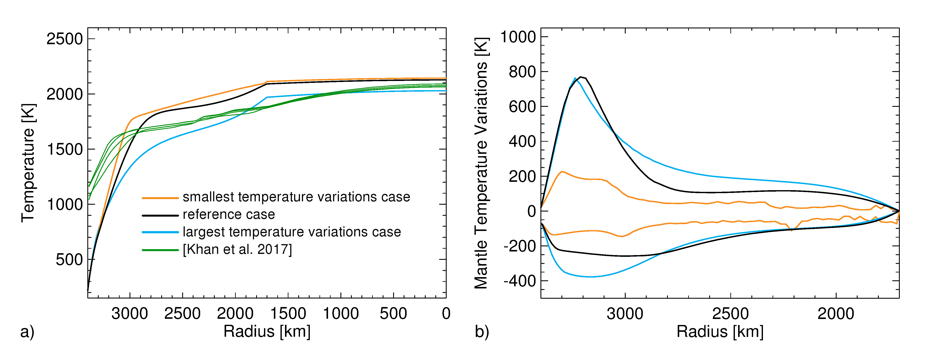
\includegraphics[width=\textwidth]
{figures/Fig4ab.png}
\caption{Panel a: temperature profiles in the mantle and core for the thermal evolution case showing the smallest temperature variations (case 8) shown in yellow color, for the thermal evolution case showing the largest temperature variations (case 27) shown in blue color and the reference case (shown in black). The temperature profiles from \citet{Khan2018} have been computed using various mantle compositions (DW, TAY, SAN and LF); Panel b: the corresponding temperature variations within the mantle as calculated from the 3D thermal evolution models by computing the difference to the average mantle temperature. Negative values indicate cold downwellings while positive values show the temperature anomaly introduced by mantle plumes.}
\label{fig:Fig4ab.png} 
\end{center}
\end{figure}
Figure 10b gives the temperature variations in the 3D calculations from the average as a function of radial distance from the CMB for the reference and the end-member models. It can be easily seen that the hot end-member model has the smallest lateral temperature variations. Upwelling and downwelling plumes are not particularly prominent. This is different for the reference model and also for the cold end-member model which both show qualitatively similar lateral variations in temperature that can reach up to 800 K at the maximum. The maxima occur partly within the thermal lithosphere. But it should be noted that the latter varies in thickness according to temperature and is comparatively thin where the temperature is large. The thermal lithosphere thickness of the reference model varies between 200 km above hot mantle plumes and up to 600 km above cold downwellings, and shows an average value of about 500 km thickness. 

The temperature of the core is little constrained. Previous models of the interior structure \citep[e.g.,][]{Sohl1997, Bertka1997, Hauck2002, Williams2004, Fei2005, Rivoldini2011, Khan2018} have assumed that the core is largely adiabatic. This would be true if the core would be vigorously convecting in which case the temperature increase in the core from the CMB to the center would amount to 200 – 300 K \citep[e.g.,][]{Sohl1997, Rivoldini2011}.  An adiabatic core will require the mantle to remove heat at a rate of at least equivalent to the heat flow conducted along the core adiabat of 5 to about 20 mW/m$^2$ \citep{Nimmo2000}. Alternatively, if the core is stably stratified, it will most likely be subadiabtic with a conductive temperature profile that matches the heat flow out of the core and the CMB temperature and has a zero heat flow in the center. We do not expect any core crystallization because core temperatures for all models are higher than the liquidus of the assumed core composition (see section 2.1).  

Our core temperature profiles assume the core to be stably stratified and are calculated to match the CMB heat flow from the detailed mantle convection calculations. In particular, 
%
\begin{equation}
T(r)=T_{CMB}+\frac{q_{CMB}}{2k_c}\left(R_c^2-r^2\right)
\end{equation} 
%    
where $T$ is temperature, $r$ radial distance from the center, $T_{CMB}$ the temperature at the CMB,  $q_{CMB}$ the heat flow there, $k_c$ the core thermal conductivity (40 W/m K) and $R_c$ the core radius. Equation (1) uses a stationary model with the cooling rate as a heat source and is a good approximation for slow secondary mantle cooling. The temperature in the core increases from the CMB to the center by some tens of Kelvin but less than 100 K. 
